\section{Lysmodul (Kristian S.)}

Lysmodulet er opbygget på fumlebræt før det blev loddet på et veroboard og modultestet.\\

\begin{figure}[h]
	\centering
	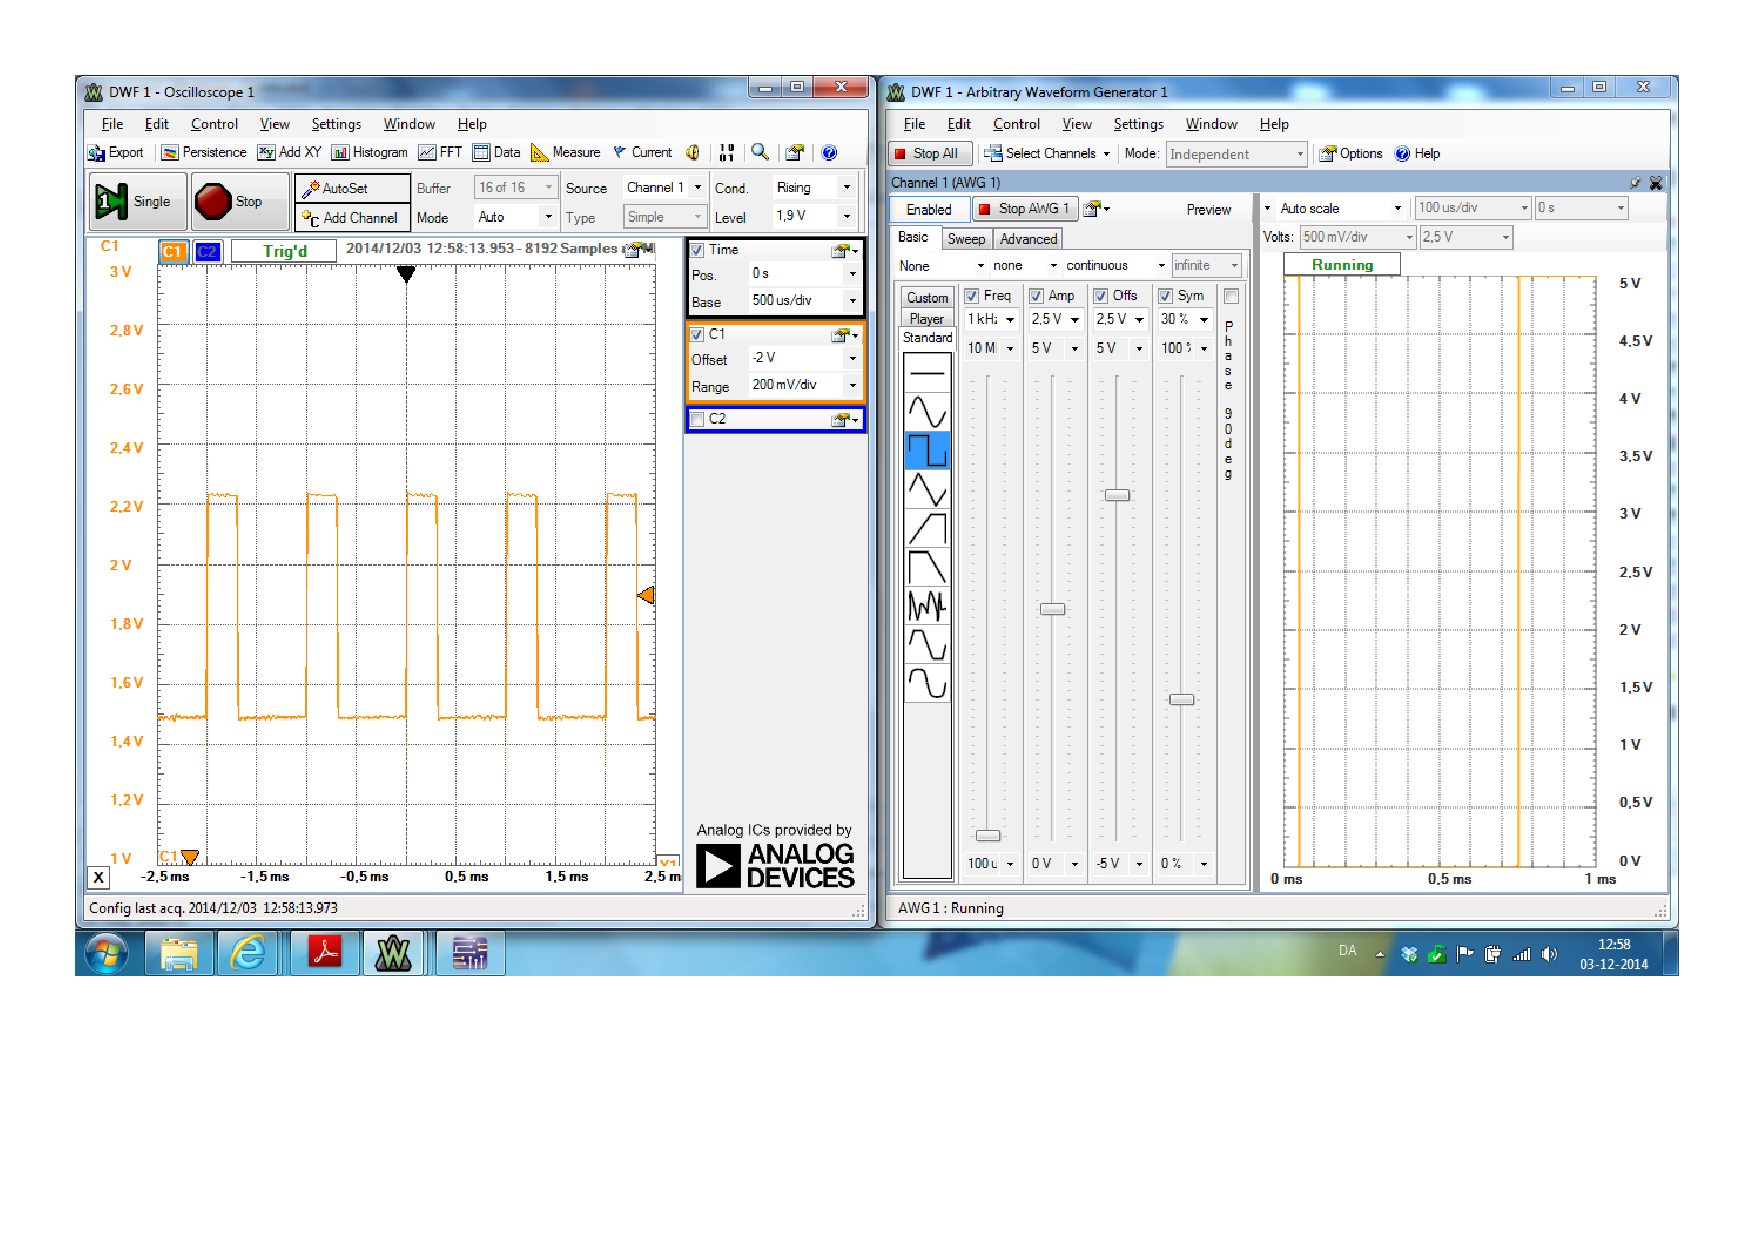
\includegraphics[width={\textwidth},trim=50 230 520 150, clip=true]{../Implementering/billeder/Waveform(30_dutycycle).pdf}
	\caption{Spænding over lysdiode, ved et $0 - 5V$ firkantsignal, med $30\%$ duty cycle}
\end{figure}

Frekvensen er valgt til $1kHz$, jf. signalbeskrivelsen på side \pageref{tbl:signalbeskriv}, eftersom en alt for lav frekvens vil give et synligt blinkende lys. Duty-cycle blev testet fra $0\%$ til $100\%$ i spring af $10\%$, og viste et tydeligt skift i lysstyrke.\\
\\
Efter test på fumlebræt blev modulet implementeret direkte på veroboard.
